\begin{columns}[totalwidth=.85\linewidth]
	\column{\textwidth}
	\vspace{-10mm}
		\begin{boxnote}
			\textbf{高分子材料でマルチマテリアル化 $\Leftrightarrow$ 高い比強度の有効利用}
                \begin{itemize}
                    \item 高分子材料の破壊耐性向上の設計指針を得たい。
                    \item 耐久性、可逆性に優れた材料としてゴム材料を選択
                \end{itemize}
			\textbf{アプローチ}
				\begin{itemize}
					% \item 実験的アプローチ
					% \begin{itemize}
					% 	\normalsize
					% 	\item 構造明確な\alert{三分岐}ネットワークを超分子で構築
					% 	\item フィラー無添加での\alert{高い破断伸びと強度}
					% 	\item 既知のモデルとの多数の整合点と、\alert{よくわからない点}。
					% \end{itemize}
					\item マルチスケールシミュレーションで\color{red}モデル\color{black}を構築
					\begin{itemize}
						\normalsize
						\item 単純化したモデルで小さなスケールから始めたい。
						\item \alert{長さの揃ったストランドで MD シミュレーション}
						% \item 最終的に、亀裂先端の挙動を FEM シミュレーション
					\end{itemize}
				\end{itemize}
			% \begin{itemize}
			% 	\item {\color{red} 「接着接合」}への高分子の利用
			% 		\begin{itemize}
			% 			\normalsize
			% 			\item 柔らかさを生かした{\color{red} 「弾性接着接合」}
			% 			\item 耐久性、可逆性に優れた\alert{ゴム材料に注目}
			% 		\end{itemize}
			% 	\item {\color{blue}耐久性が不明確}
			% 		\begin{itemize}
			% 			\normalsize
			% 			\item とくに疲労破壊に対して
			% 		\end{itemize}
			% \end{itemize}
		\end{boxnote}

		\begin{itembox}[l]{古典ゴム弾性理論でのミクロな変形モデル}
			\begin{columns}[T, onlytextwidth]
				\column{.48\linewidth}
					\begin{itembox}[l]{Affine Network Model}
						\begin{itemize}
							\item 架橋点の Affine 変形を仮定
								\begin{align*}
									\sigma_{nom} &= \textcolor{red}{\nu} k_B T \left(\lambda - \dfrac{1}{\lambda^2}\right) \\
									&= G_{affine} \left(\lambda - \dfrac{1}{\lambda^2}\right)
								\end{align*}
						\end{itemize}
					\end{itembox}
				\column{.48\linewidth}
					\begin{itembox}[l]{Phantom Network Model}
						\begin{itemize}
							\item \alert{架橋点ゆらぎ}を考慮
							\item 架橋点の分岐数 $f$
						\end{itemize}
						% \vspace{-2mm}
						% \small
						\begin{align*}
							G_{phantom} &= \nu k_B T \left(1 - \dfrac{2}{f}\right) \\
						\end{align*}
					\end{itembox}
			\end{columns}     
		\end{itembox}



		% \begin{itembox}[l]{ヒステリシスと破壊靭性}
		% 	\begin{columns}[totalwidth=\linewidth]
		% 		\column{.75\textwidth}
		% 			\begin{itemize}
		% 				\item 力学的ヒステリシス
		% 				\begin{itemize}
		% 					\normalsize
		% 					\item
		% 					\textcolor{blue}{loading} 時に比べて、\textcolor{red}{Unloading} 時の応力が低下
		% 					\item
		% 					ヒステリシスロス:変形時のエネルギー散逸
		% 				\end{itemize}
		% 				\item 破壊靭性との関係
		% 				\begin{itemize}
		% 					\normalsize
		% 					\item
		% 					Andrews 理論:ヒステリシスロスの重要性が指摘
		% 				\end{itemize}
		% 			\end{itemize}
		% 		\column{.25\textwidth}
		% 			\centering
		% 			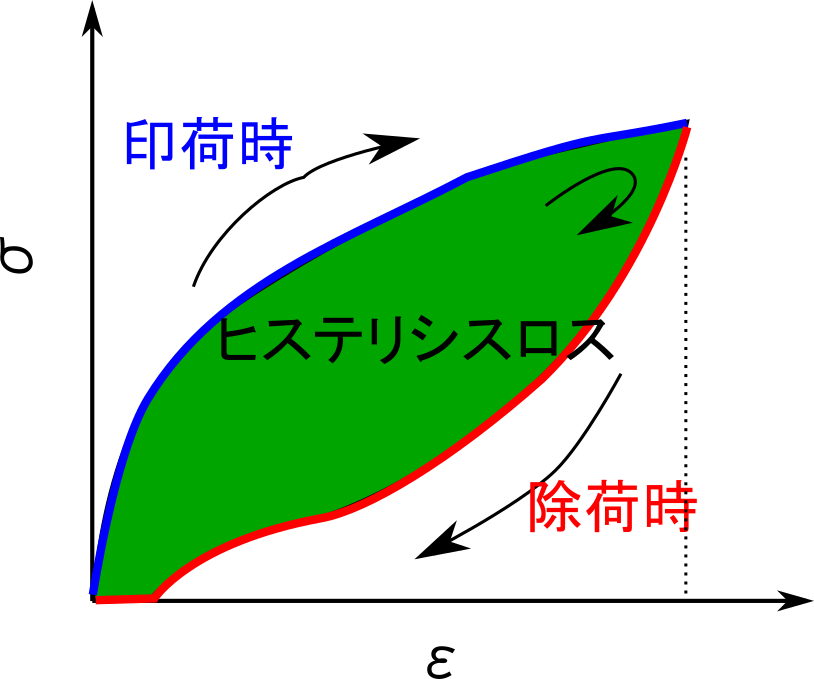
\includegraphics[width=\textwidth]{hysteresis_curve.png}
		% 		\end{columns}
		% \end{itembox}

		% \begin{itembox}[l]{Andrews 理論\cite{andrews}}
		% 	\begin{columns}[totalwidth=\textwidth]
		% 		\column{.8\textwidth}
		% 			クラックの微小進展時に、
		% 			\begin{itemize}
		% 				\item
		% 				\textcolor{blue}{Loading 場}と\textcolor{red}{Unloading 場}のひずみエネルギーの差
		% 				\item
		% 				全体の変形に要したエネルギーの多くを\textcolor{red}{散逸}
		% 				\item
		% 				鎖の破断へのエネルギーが低減 $\Rightarrow$ \alert{強靭さの起源。}
		% 			\end{itemize}	
		% 		\column{.2\textwidth}
		% 			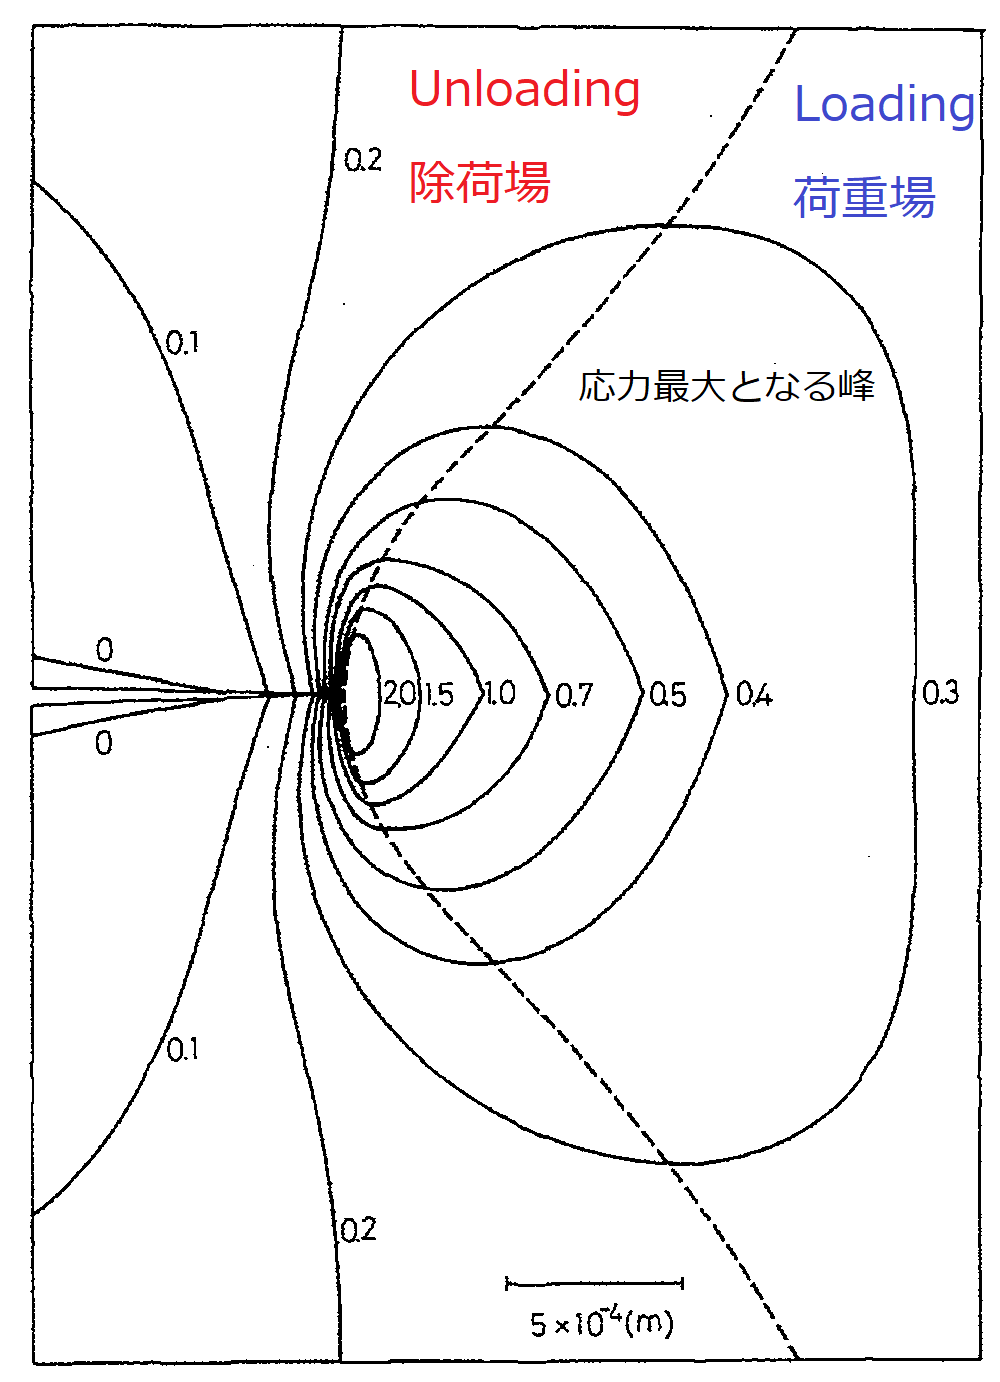
\includegraphics[width=.85\textwidth]{crack.png}     
		% 	\end{columns}
		% \end{itembox}

		% \begin{itembox}[l]{ゴムの破断強度の時間温度依存}
		% 	\begin{columns}[totalwidth=\textwidth]
		% 		\column{.5\textwidth}
		% 			\alert{粘弾性極限}\cite{lake}(高温・低速)
		% 		\column{.5\textwidth}
		% 			変形速度、温度\cite{smith} で\alert{破壊包絡線}
		% 	\end{columns}
		% 	\begin{columns}[totalwidth=\textwidth]
		% 		\column{.5\textwidth}
		% 			\centering
		% 			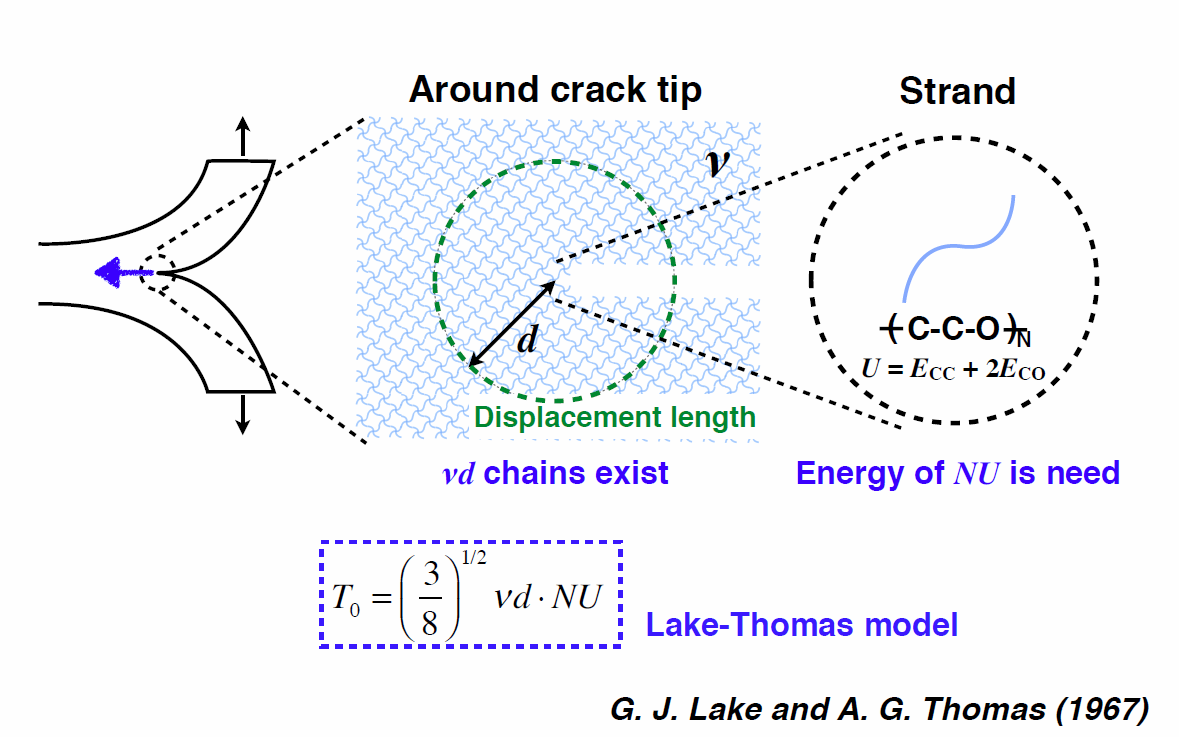
\includegraphics[width=.8\textwidth]{Lake_Thomas.png}
		% 		\column{.25\textwidth}
		% 			\centering
		% 			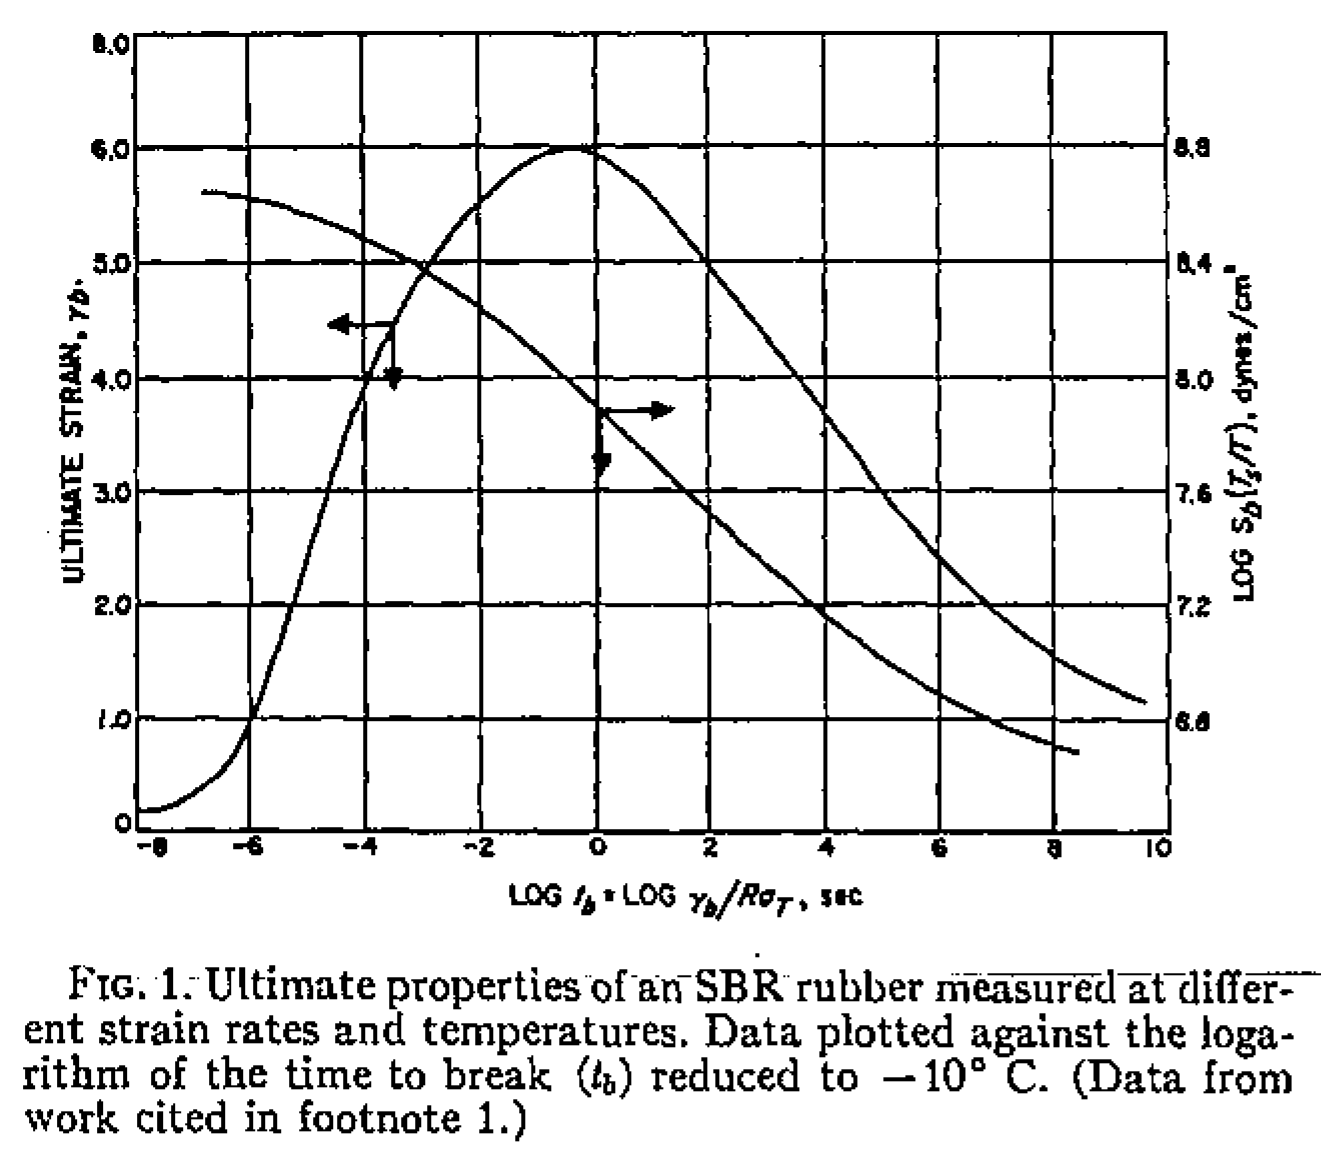
\includegraphics[width=.9\textwidth]{Time_Temp_2.png}
		% 		\column{.25\textwidth}
		% 			\centering
		% 			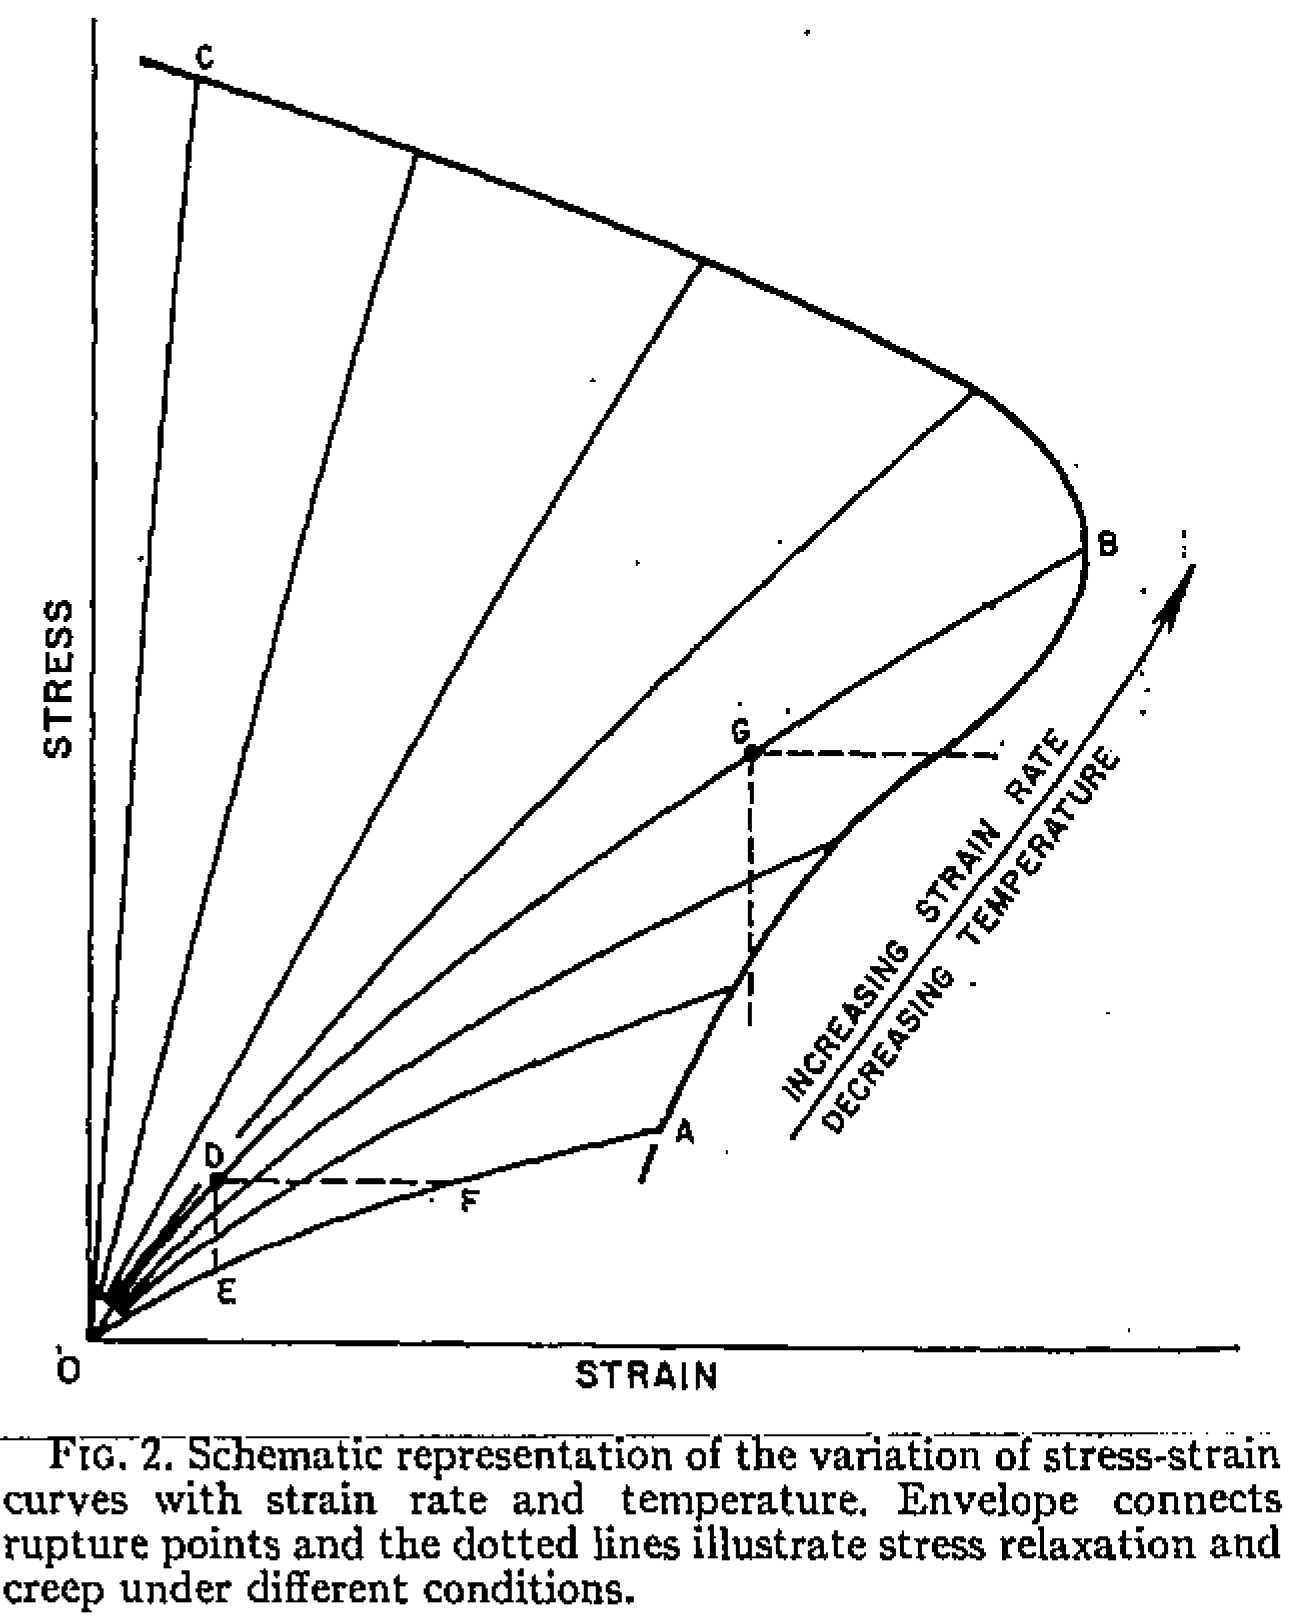
\includegraphics[width=.7\textwidth]{Time_Temp_3.png}
		% 	\end{columns}
		% \end{itembox}

		\begin{itembox}[l]{架橋点の環境とランダムな接続性\cite{flory}}
			\begin{columns}[totalwidth=\textwidth]
				% \column{.35\textwidth}
				% \centering
				% 	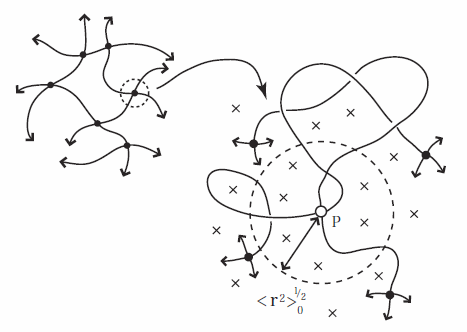
\includegraphics[width=.8\textwidth]{JP_vicinity.png}

				% 	\small
				% 	架橋点は\alert{多数のストランド}に\\囲まれている。
				\column{.55\textwidth}
					\begin{itemize}
						\item 接続性を不均一に
							\begin{itemize}
								\normalsize
							    \item 接続に\alert{位置依存性}
							\end{itemize}
						\item 巨視的な変形後
							\begin{itemize}
								\normalsize
								\item \alert{結節点のゆらぎが\\不均一}
								\item 多様な緩和モード
								% \item \alert{緩和の長時間化?}
							\item \alert{Phantom Network の\\諸特性が発現}
							\end{itemize}
					\end{itemize}
				\column{.4\textwidth}
					\centering
					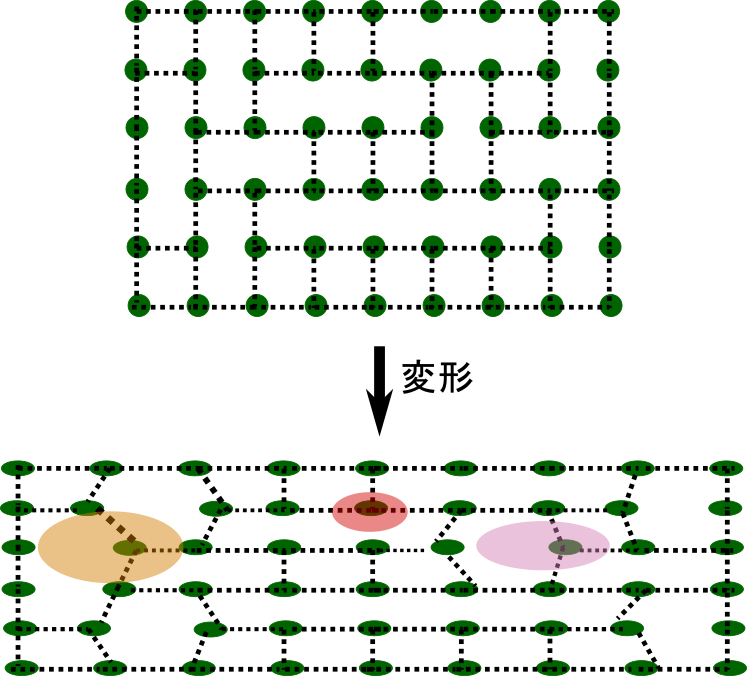
\includegraphics[width=\textwidth]{random_NW.png}
			\end{columns}
		\end{itembox}
\end{columns}